\section{Obervations and Data Reduction}

\subsection{Observation Region}
The Orion region consists of two giant molecular clouds, the Orion A and B clouds. This research covers the Orion A Cloud. The Orion A Cloud covers about $29 \, \textrm{deg}^2$ of the sky and its distance is about 450$\,$pc \cite{kounkel2017gould}. The total mass is estimated to be about $10^5 \, M_{\odot}$. It contains several hot molecular cores, such as the BN-KL nebula. It is known that the Orion Cloud was formed by a collision and fragmentation between two giant molecular clouds about 60 million years ago. The effects of the collision can be seen nowdays. There is a big velocity gradient along the declination axis. On the north side of the Orion A Cloud (OMC 2) shows about 12$\, \rm km\,s^{-1}$ but on the south end (L1641) it has velocity about 5$\, \rm km\,s^{-1}$ \cite{schulz2012formation}.

\subsection{Observation Data}
%%% 박기현 수정 시작
The $^{12}\textrm{CO (J = 2 - 1, 230.538\,GHz)}$ data was observed with the IRAM $\textrm{30\,m}$ telescope in Granada, Spain, in 2013. The spatial beamwidth was $\textrm 11^{\prime\prime}$, and the spectral resolution was 0.4$\, \rm km\,s^{-1}$. The noise level was 0.2$\, \rm K$. It only covers the north region of the Orion A cloud \cite{berne2014iram}.

The $^{12}\textrm{CO (J = 1 - 0, 115.271\,GHz})$ data was observed with the NRO 45m telescope in Nobeyama, Japan.

The $^{13}\textrm{CO (J = 1 - 0, 110.201\,GHz})$ and the $\textrm{C}^{18}\textrm{O (J = 1 - 0, 109.782\,GHz})$ data were observed at Taeduk Radio Astronomy Observatory (TRAO)  $\textrm{13.7\,m}$ telescope in 2017. The spatial beamwidth was $\textrm 45^{\prime\prime}$, and the spectral resolution was 0.05$\, \rm km\,s^{-1}$. The noise level was 0.4$\,$K.\\
$^{13}\textrm{CO}$ and $\textrm{C}^{18}\textrm{O}$ lines are optically thin lines which can trace most of the matter on the line of sight, contrasting to $^{12}\textrm{CO}$ lines which are so optically oblique that it can only trace the outermost part of the molecular core. In this study, I used TRAO data to determine the protostar's velocity and linewidth which are the kinematic properties of the envelope. Then, I will trace the outflow jets using $^{12}$CO data.
%%%박기현 수정 끝

%%%선재 원본
%%%The $^{12}$CO(J = 2 - 1, $230.538\,\rm GHz$) data was observed with the IRAM 30$\,$m telescope in Granada, Spain, in 2013. The spatial beamwidth was 11", and the spectral resolution was 0.4$\, \rm km\,s^{-1}$. The noise level was 0.2$\, \rm K$. It only covers the north region of the Orion A cloud \cite{berne2014iram}. \\
%%%The $^{12}$CO (J = 1 - 0, $115.271\, \rm GHz$) data was observed with the NRO 45m telescope in Nobeyama, Japan.  \\
%%%The $^{13}$CO (J = 1 - 0, $110.201\,$GHz) and the $\textrm{C}^{18}\textrm{O}$(J = 1 - 0, 109.782 GHz) was observed at Taeduk Radio Astronomy Observatory (TRAO) 13.7$\,$m telescope in 2017. The spatial beamwidth was 45", and the spectral resolution was 0.05$\, \rm km\,s^{-1}$. The noise level was 0.4$\,$K.\\
%%%$^{13}$CO and $\textrm{C}^{18}\textrm{O}$ lines are optically thin lines which can trace most of the matter on the line of sight, contrasting to $^{12}$CO lines which are so optically oblique that it can only trace the outermost part of the molecular core. In this study, I used TRAO data to determine the protostar's velocity and linewidth which are the kinematic properties of the envelope. Then, I will trace the outflow jets using $^{12}$CO data.

Figure \ref{fig:map1} shows the data from IRAM and TRAO. The intensity of the $^{12}\textrm{CO}$ data is approximately 10 times stronger than the $^{13}\textrm{CO}$ data.

%\begin{figure}[h]
\begin{figure}[t]
	\begin{center}
		\begin{tabular}{cc}
			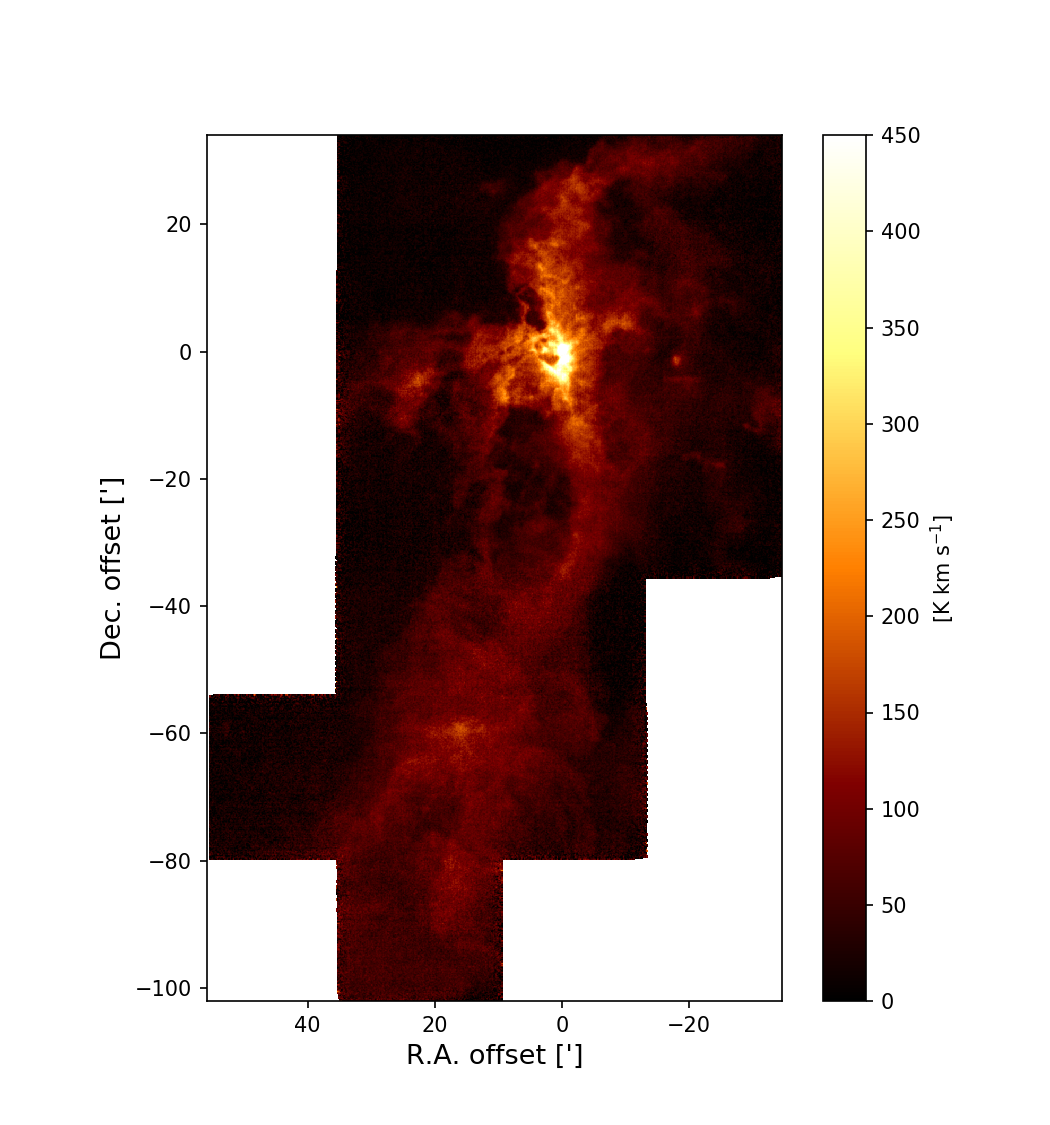
\includegraphics[width=0.45\textwidth]{RNE_12CO_Orion} & 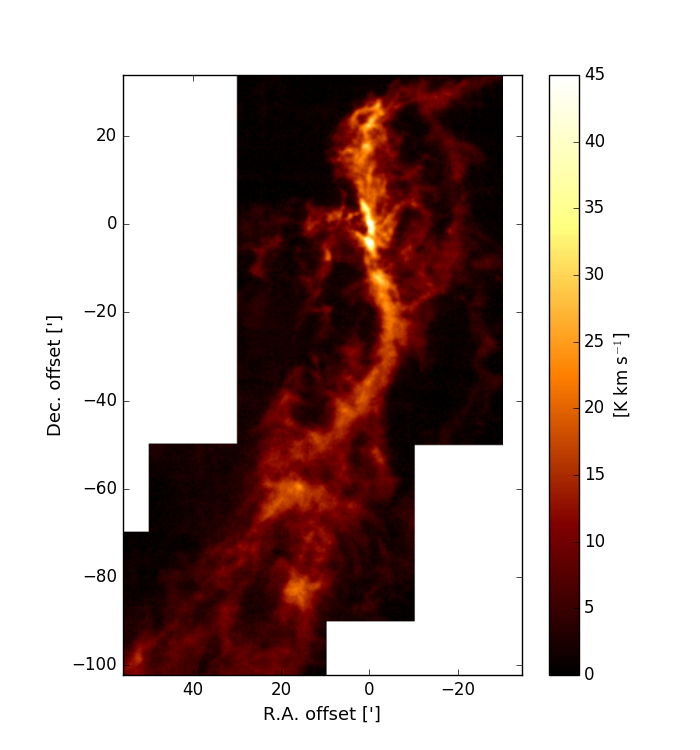
\includegraphics[width=0.45\textwidth]{Orion_13CO_intmap}
		\end{tabular}
	\end{center}
	\caption{Orion A $^{12}$CO (J = 2 - 1) integrated intensity map(left) $^{13}$CO integrated intensity map(right).}
	\label{fig:map1}  %%%박기현샘 추가함 (이렇게 넣어야 제데로 ref 됨.)
	%%% 박기현 레이블을 달고, 본문에서 언급하면 latex에서 알아서 같은 페이지로 보내줌.
\end{figure}

\subsection{Identification of Outflows}
Data obtained by observing with radio waves are summed over the line of sight, which tells us the distribution of matter which has relative radial velocity to the observer. The envelope around the protostar is static or is contracting slowly to the protostar itself, but outflow jets have big velocity components from each pole. If the inclination of the outflows are not zero, it would be seen as jets are moving closer or further from the observer. In this study, $^{13}$CO and $\textrm{C}^{18}\textrm{O}$ lines were used to get the velocity distribution of the protostar. By using Gaussian fitting, I calculated the protostar’s central velocity($v_{cen}$) and the full width at half maximum (FWHM). The intervals of the red/blue lobes were defined by how far is it from the center velocity and how strong the intensity is.

Because the emission lines of $^{12}$CO are optically thicker than other lines, it is appropriate to trace the outflows with $^{12}$CO lines. I drew contour maps to find out if bipolar outflows existed with the protostar at its center. To check if the red blue lobes that are found are outflows from the same protostar I checked the $^{12}$CO, $^{13}$CO, $\textrm{C}^{18}\textrm{O}$ lines from the red peak, blue peak, and the center points. For each outflows confirmed, I calculated the column density and the momentum force.

The column density can be calculated as the following expression:
\begin{align}
	N_{H_2} =& \frac{8\pi \nu^3}{c^3} \frac{1}{(2J_l +3)A}  \notag \\
	& \times \frac{Z(T_{ex})}{exp(-E_l / kT_{ex})[1-exp(h\nu / kT_{ex})]} \notag \\
	& \times \frac{\int T_B dV}{J(T_{ex})-J(T_{bg})}
\end{align}

\begin{equation}
J(T) = \frac{h \nu / k}{exp(h\nu / kT)-1}
\end{equation}

In the above equation, $\nu$ is the corresponding frequency of emission line, $c$ is the speed of light, $J_l$ is the rotational quantum number of the lower energy level, $A$ is the Einstein A coefficient, $Z$ is the partition function, $E_l$ is the rotational energy of the lower energy level, $k$ is the Boltzmann's constant, $T_{ex}$ is the excitation temperature of the transitions, $\int T_B dV$ is the integrated intensity measured, $T_{bg}$ is the background radiation temperature. I assumed a local thermal equilibrium(LTE) excitation at an outflow temperature of 50$\,$K \cite{takahashi2008millimeter}.\\

The mass within one beam can be calculated as the following:

\begin{equation}
M_B =  \frac{\pi}{4} D^2 \theta_B ^2 X[\textrm{CO}] N_{\textrm{H}_2} m_{\textrm{H}_2}
\end{equation}

$D$ is the distance to the objects, $\theta_B$ is the beam size, $m_{\textrm{H}_2}$ is the mass of one hydrogen molecule. $X[\textrm{CO}]$ is the abundance ratio of CO to $\textrm{H}_2$. In this paper, $D = 450\,\textrm{pc}$ and $X[\textrm{CO}] = 10^{-4}$ was used \cite{hatchell2007star}.\\

\subsection{Calculating Momentum Flux}

The momentum flux within one beam is calculated as the following:

\begin{equation}
\dot{P} = \frac{dP}{dt} = \sum_{v} {\frac{M_B (v) (v/ \cos i)}{D\theta_B / (v \tan i)}}
\end{equation}

$v$ is the velocity offset from $v_{cen}$, $M_B (v)$ is the mass within one beam, $i$ is the inclination within one beam \cite{hatchell2007star}.
Then the momentum flux from individual beams are summed in annuli. 

\begin{equation}
F_{\textrm{CO}} = \sum _{annulus} \frac{2\pi \theta_r}{N_{pix}\theta_B}\dot{P}	
\end{equation}

$N_{pix}$ is the number of pixels in a annulus. $\theta_r$ is the distance between each pixel and the outflow center. $\theta_B$ is the beam size \cite{hatchell2007star, van2013outflow}.
